\documentclass[11pt]{article}
\usepackage[margin=1in]{geometry}
\usepackage{amsmath,amssymb,amsthm,bm}
\usepackage{booktabs}
\usepackage{hyperref}
\usepackage{xcolor}
\usepackage{tikz}
\usetikzlibrary{positioning,arrows.meta}
\hypersetup{colorlinks=true,linkcolor=blue!50!black,citecolor=blue!50!black,urlcolor=blue!50!black}

\newtheorem{assumption}{Assumption}
\theoremstyle{remark}
\newtheorem{remark}{Remark}
\theoremstyle{definition}
\newtheorem{definition}{Definition}

\newcommand{\R}{\mathbb{R}}
\newcommand{\x}{\bm{x}}
\newcommand{\uu}{\bm{u}}
\newcommand{\bU}{\bm{U}}
\newcommand{\q}{\bm{q}}
\newcommand{\qd}{\dot{\bm{q}}}
\newcommand{\qdd}{\ddot{\bm{q}}}
\newcommand{\btau}{\bm{\tau}}
\newcommand{\blam}{\bm{\lambda}}
\newcommand{\f}{\bm{f}}
\newcommand{\p}{\bm{p}}
\newcommand{\n}{\bm{n}}
\newcommand{\cc}{\bm{c}}
\newcommand{\J}{\bm{J}}
\newcommand{\Rot}{\bm{R}}
\newcommand{\I}{\bm{I}}
\newcommand{\zero}{\bm{0}}
\newcommand{\skewm}[1]{[#1]_\times}
\newcommand{\code}[1]{\texttt{#1}}
\DeclareMathOperator{\clip}{clip}
\DeclareMathOperator{\wrap}{wrap}
\DeclareMathOperator{\atantwo}{atan2}
\DeclareMathOperator{\Log}{Log}

\title{ALIP-MPC Whole-Body Locomanipulation:\\ Technical Notes}
\author{}
\date{\today}

\begin{document}
\maketitle

\begin{abstract}

\end{abstract}

\tableofcontents

%=======================================================================
\section{System overview}\label{sec:overview}
%=======================================================================
The goal of this project is whole-body loco-manipulation on a humanoid: the robot must walk up to a large
object (currently a box), make contact with its hands, and push it to a goal pose in $SE(3)$ while staying balanced.
The task mixes two kinds of decisions:
\begin{itemize}
  \item \textbf{Discrete, long-horizon decisions}: where to touch the object, when to let go and touch somewhere
        else, and which intermediate pose the object should reach next.
  \item \textbf{Continuous, short-horizon control}: where to place the next footstep, how hard each hand should
        push, and which joint torques realize all of this without falling or slipping.
\end{itemize}
These are handled by separate layers. Each layer runs at its own rate and passes a small, well-defined quantity to
the layer below it. The controller of Gibson et al.~\cite{gibson2022} provides the locomotion core. This work
extends it with hand-contact forces and puts a contact planner on top.

\subsection{Control hierarchy}
\begin{center}
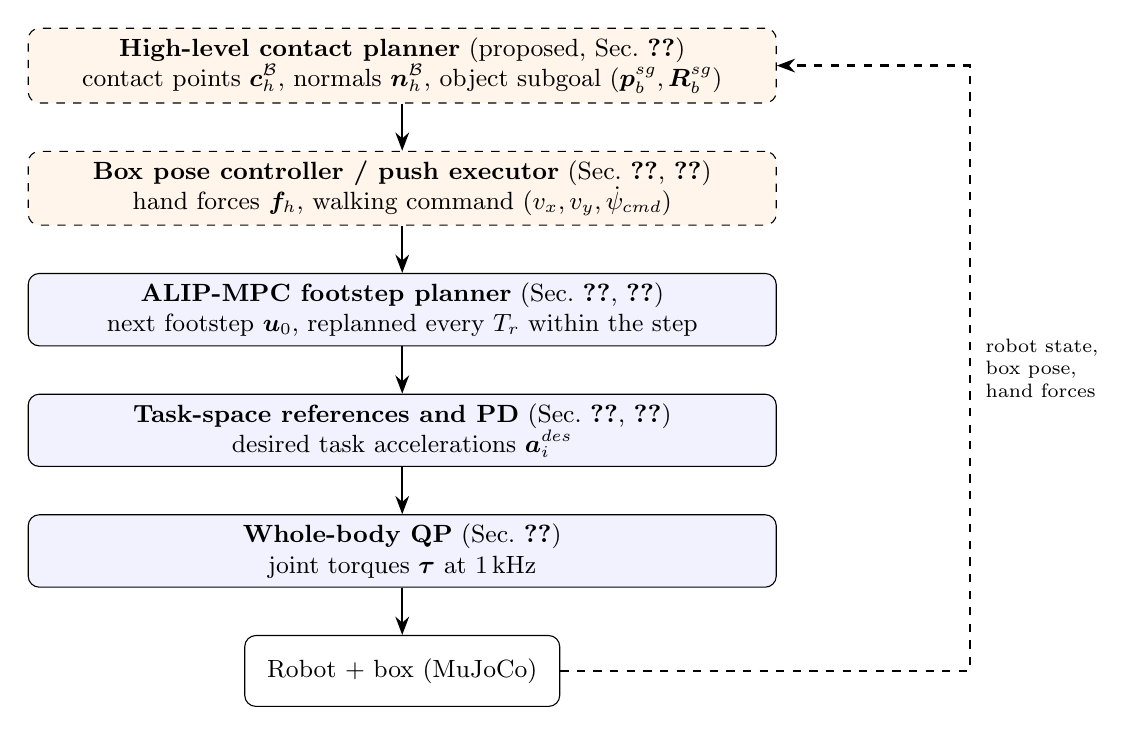
\begin{tikzpicture}[
    node distance=6mm,
    blk/.style={draw, rounded corners, align=center, minimum width=9.5cm, minimum height=9mm, font=\small},
    prop/.style={blk, dashed, fill=orange!8},
    impl/.style={blk, fill=blue!5},
    arr/.style={-{Stealth}, thick},
    lab/.style={font=\scriptsize, align=left, right=2pt}]
  \node[prop] (hl)  {\textbf{High-level contact planner} (proposed, Sec.~\ref{sec:hlplanner})\\
                     contact points $\cc_h^{\mathcal B}$, normals $\n_h^{\mathcal B}$, object subgoal $(\p_b^{sg},\Rot_b^{sg})$};
  \node[prop, below=of hl] (bp) {\textbf{Box pose controller / push executor} (Sec.~\ref{sec:push}, \ref{sec:boxpose})\\
                     hand forces $\f_h$, walking command $(v_x,v_y,\dot\psi_{cmd})$};
  \node[impl, below=of bp] (mpc) {\textbf{ALIP-MPC footstep planner} (Sec.~\ref{sec:alip}, \ref{sec:alipforce})\\
                     next footstep $\uu_0$, replanned every $T_r$ within the step};
  \node[impl, below=of mpc] (ref) {\textbf{Task-space references and PD} (Sec.~\ref{sec:taskref}, \ref{sec:pd})\\
                     desired task accelerations $\bm a_i^{des}$};
  \node[impl, below=of ref] (wbc) {\textbf{Whole-body QP} (Sec.~\ref{sec:wbc})\\
                     joint torques $\btau$ at $1\,$kHz};
  \node[blk, below=of wbc, minimum width=4cm] (sim) {Robot + box (MuJoCo)};
  \draw[arr] (hl) -- (bp);
  \draw[arr] (bp) -- (mpc);
  \draw[arr] (mpc) -- (ref);
  \draw[arr] (ref) -- (wbc);
  \draw[arr] (wbc) -- (sim);
  \draw[arr, dashed] (sim.east) -- ++(5.2,0) |- node[lab, pos=0.25] {robot state,\\box pose,\\hand forces} (hl.east);
\end{tikzpicture}
\end{center}
Blue boxes are implemented. Dashed orange boxes are proposed or only partly working. From top to bottom:
\begin{enumerate}
  \item \textbf{High-level contact planner} (event-driven, once per contact phase). It chooses a \emph{contact
        intention}: one contact point per hand on the object surface and a subgoal pose that the object should reach
        while those contacts are held. A hand-written heuristic stands in for it at the moment
        (\code{HeuristicIntentionPlanner} in \code{intention.py}). The goal is to replace it with a learned policy.
  \item \textbf{Box pose controller / push executor} (every control step). It turns the intention into
        (i) the planned hand forces $\f_h$ needed to move the box toward the subgoal, (ii) hand position targets that
        realize those forces through depth admittance, and (iii) a walking command that keeps the torso behind the
        hands. 
        
        \textbf{Currently:} the contacts and push direction are fixed, and only the open-loop force planner works
        (Section~\ref{sec:push}).
  \item \textbf{ALIP-MPC} (once per foot step, re-solved every $T_r$ during the step). It picks footstep locations that track
        the commanded velocity. The planned hand forces enter its dynamics as the moment $\btau$ about the stance foot,
        and the reference orbit is shifted so the robot leans into the push (Section~\ref{sec:alipforce}).
  \item \textbf{Task-space references and PD} (every control step). These interpolate swing-foot, torso and hand
        trajectories between the discrete MPC outputs and turn tracking errors into desired accelerations.
  \item \textbf{Whole-body QP} ($1\,$kHz). It solves for $(\qdd,\blam)$ subject to the floating-base dynamics with the
        \emph{planned} hand forces, friction and torque limits, then recovers the torques $\btau$.
\end{enumerate}

\paragraph{One shared hand force.} The planned hand force $\f_h$ is the main link between manipulation and locomotion.
The same value is used (a) as the force set-point of the depth-admittance loop, (b) as a known external wrench in the WBC
dynamics~\eqref{eq:fbdyn}, and (c) as the disturbance moment $\btau$ in the ALIP-MPC~\eqref{eq:pushtau}. Because all
three agree, the footstep planner already expects the push, the WBC already compensates for it, and the hands are
regulated to produce it.

\paragraph{Separation of concerns.} The ALIP-MPC never reasons about the task. It sees only a velocity command and
a predicted external moment. The contact planner never reasons about balance or footsteps. It sees only object poses
and contact locations. This keeps every layer small: the MPC remains a dense QP with $2H$ variables, and the planner's
action space stays low-dimensional, which makes it suitable for learning.

\subsection{High-level contact planner (proposed)}\label{sec:hlplanner}
\paragraph{Motivation.} With fixed contacts, the robot can only push the box along a direction that the chosen face
supports. A large heading change, or a goal behind or beside the box, cannot be reached from a single face within the
hand force limits: with hand spacing $s=0.5\,$m the hands cannot rotate the box in place within $f_{\max}=60\,$N. The robot must release the box, walk to a new
side, and touch it again. Choosing these contacts is a discrete, long-horizon problem that the continuous layers below
are not designed to solve.

\paragraph{Approach.} Following \emph{Where to Touch, How to Contact} (Xie et al.~\cite{xie}), the high-level action
is a contact intention
\begin{equation}
  \mathcal I=\big(\cc_r,\,\cc_l,\ \n_r,\,\n_l,\ \p_b^{sg},\,\Rot_b^{sg}\big),
  \label{eq:intention}
\end{equation}
where $\cc_i$ is the contact position, and $\n_i$ is the normal vector of contact $i$, and $\p_b^{sg},\,\Rot_b^{sg}\big)$ are the desired position and orientation of the object after these contacts. 
This intention represets where to touch the object (from the contact points and outward normals in the object frame) and \emph{what the
object should do} after contact (a subgoal pose in the world frame). To keep the action space small and discrete, the
contact points will be chosen from a fixed grid of keypoints sampled on the faces of the box
The planner observes the current object pose, the final goal pose and the robot state, and outputs~\eqref{eq:intention}.
The low-level stack executes the intention using the MPC-WBC formulation. The planner does not choose footsteps, forces or torques.

\paragraph{Execution of one contact phase.}
\begin{enumerate}
  \item \textbf{Plan.} Query the planner for $\mathcal I$ given the current object pose and the final goal.
  \item \textbf{Approach.} Walk to a stand-off pose behind the selected contacts, facing the contact face. This is
        plain velocity tracking with the ALIP-MPC (the hands carry no force, so $\btau=\zero$).
  \item \textbf{Engage.} Move the hands to $\cc_h$ and ramp the planned force $\f_h$ up from zero, so that the MPC
        moment $\btau$ and the orbit shift $(\Delta x_c,\Delta y_c)$ grow smoothly rather than jumping.
  \item \textbf{Push.} The box pose controller drives the object toward $(\p_b^{sg},\Rot_b^{sg})$: it chooses the
        hand force split and the walking command, and the ALIP-MPC and WBC carry them out.
  \item \textbf{Release.} When the subgoal is reached, or progress stalls, ramp $\f_h$ down to zero, lift the hands
        off, and return to step 1. The task ends when the final goal is reached.
\end{enumerate}

\paragraph{Intermediate Step} Before implementing the RL policy to output these intentions, I want to build a  simple planner that outputs the same contact intentions using first principles. 

\paragraph{Open questions.}
\begin{itemize}
  \item \textbf{Training.} Train the policy with RL in simulation with the full low-level stack in the loop (slow, but
        it learns what the controller can actually do), or with a cheaper surrogate of the push dynamics first. Will need to parallelize MPC controller in order to run in RL training
  \item \textbf{Feasibility.} Only intentions the low level can execute should be offered: contact heights within arm
        reach (push at about $1.35\,$m), sliding before tipping ($\mu_b h<$ half width), and subgoals reachable within the
        hand force limits. These can be enforced by masking the action set or learned through the reward.
  \item \textbf{Contact switching.} When contact is made or released, the step in $\btau$ changes the MPC equilibrium
        $\bar\x$ (Section~\ref{sec:shift}). Ramping the force over one or two steps should keep the footstep planner
        within its reach constraint $\bar u$.
\end{itemize}

%=======================================================================
\section{ALIP model}\label{sec:alip}
%=======================================================================
\subsection{Related Work}
Locomotion controller inspired by Gibson et al paper \cite{gibson_terrain-adaptive_2022}

\subsection{Continuous dynamics}
The ALIP state is
\begin{equation}
  \x=\begin{bmatrix}x_c & y_c & L_x & L_y\end{bmatrix}^\top,
\end{equation}
where $(x_c,y_c)$ is the horizontal CoM position relative to the stance foot and
$\bm L=(L_x,L_y)$ is the horizontal angular momentum about the contact point:
\begin{equation}
  \bm L_{c}=\bm L_{G}+\bm r\times m\,\bm \dot{\p}_{G},\qquad \bm r=\p_{G}-\p_{st},
  \label{eq:Lcontact}
\end{equation}
with $\bm L_G$ the centroidal angular momentum and $\bm p_G$ is the position of the CoM in the world frame and $\bm p_{st}$ is the position of the stance foot. Both $\bm r$ and $\bm L_c$
are rotated into the inertial frame, $\mathcal S$ of the robot, by $\Rot_{st}^\top$.

\begin{assumption}[ALIP]\label{as:alip}
(i) The CoM height is constant, $z_G\equiv z_H$. (ii) The stance contact is a point: the
contact applies no moment, and there are no other external forces. (iii) In the kinematic relation between
$\bm L_c$ and the CoM velocity, the centroidal term $\bm L_G$ is neglected.
\end{assumption}

Under (ii), the angular momentum balance about the contact point is \emph{exact}:
$\dot{\bm L}_c=\bm r\times(-mg\,\bm e_z)$, so $\dot L_x=-mg\,y_c$ and $\dot L_y=mg\,x_c$. Under (i) and (iii),
\eqref{eq:Lcontact} gives $\bm L_c\approx m z_H(-\dot y_c,\ \dot x_c)$. This is the advantage of the ALIP over the LIP:
the approximation affects only the kinematic rows, while $\bm L_c$ is measured including $\bm L_G$ \cite{gibson2022}.
Together, these give the linear system
\begin{equation}
  \dot\x=A\x,\qquad
  A=\begin{bmatrix}
  0 & 0 & 0 & \frac{1}{m z_H}\\
  0 & 0 & -\frac{1}{m z_H} & 0\\
  0 & -mg & 0 & 0\\
  mg & 0 & 0 & 0
  \end{bmatrix}.
  \label{eq:alipA}
\end{equation}
The sagittal pair $(x_c,L_y)$ and the lateral pair $(y_c,L_x)$ decouple. With
$\ell=\sqrt{g/z_H}$, the sagittal flow is
\begin{equation}
  \begin{bmatrix}x_c(t)\\L_y(t)\end{bmatrix}=
  \begin{bmatrix}\cosh\ell t & \frac{\sinh\ell t}{m z_H\ell}\\ m z_H\ell\sinh\ell t & \cosh\ell t\end{bmatrix}
  \begin{bmatrix}x_c(0)\\L_y(0)\end{bmatrix},
  \label{eq:flow}
\end{equation}
and the lateral flow has the same form with $(x_c,L_y)\to(y_c,-L_x)$.

\subsection{Step-to-step map}
The step duration, $T_s$ is fixed. The descretized inter-step dynamics can be written as $A_d=e^{AT_s}$.
At touchdown, the swing foot lands at $\uu=(u_x,u_y)$ relative to the old stance foot (in $\mathcal S$).
The CoM position is re-measured from the new foot, and $\bm L_c$ is continuous at impact
under the point-contact, no-impulse assumption, because the new contact passes through the
same horizontal plane:
\begin{equation}
  \x^+=\x^-+B\uu,\qquad B=\begin{bmatrix}-\I_2\\ \zero_{2\times2}\end{bmatrix}.
  \label{eq:impact}
\end{equation}
\begin{remark}
From \eqref{eq:Lcontact}, $\bm L$ about the new contact is $\bm L_{new}=\bm L_{old}-\bm u\times m\bm v_G$. For a horizontal
$\bm u=(u_x,u_y,0)$, the horizontal part of $\bm u\times\bm v_G$ is $\dot z_G\,(u_y,-u_x)$, which vanishes under
Assumption~\ref{as:alip}(i). With no impulsive contact force (the swing foot lands with no impact), $\bm L_c$ is
then continuous, and \eqref{eq:impact} is exact within the model.
\end{remark}
Propagate-then-impact (\code{step\_transition}) gives the discrete step map from the
post-impact state of step $k$ to that of step $k+1$:
\begin{equation}
  \x_{k+1}=A_d\x_k+B\uu_k.
  \label{eq:dstep}
\end{equation}

\subsection{Horizon prediction}
For a prediction horizon of $H$ footsteps, the states and inputs are stacked into 
$\bU=(\uu_0,\dots,\uu_{H-1})\in\R^{2H}$ and $\bm X=(\x_1,\dots,\x_H)\in\R^{4H}$. Iterating
\eqref{eq:dstep}:
\begin{equation}
  \bm X=\Phi\,\x_0+\Gamma\,\bU,\qquad
  \Phi=\begin{bmatrix}A_d\\A_d^2\\ \vdots\\ A_d^H\end{bmatrix},\quad
  \Gamma_{ij}=\begin{cases}A_d^{\,i-j}B & j\le i\\ \zero & j>i\end{cases}
  \quad(i,j=0,\dots,H-1).
  \label{eq:stack}
\end{equation}
Block row $i$ of $\bm X$ is the post-impact state after $i+1$ steps.

\subsection{QP-MPC Formulation}
\begin{equation}
\begin{aligned}
  \min_{\bU}\ \ & (\bm X-\bm X_{ref})^\top Q\,(\bm X-\bm X_{ref})+R\,\|\bU\|^2\\
  \text{s.t.}\ \ & -\bar u\le u_{x,k}\le\bar u,\\
  & \sigma_k\,u_{y,k}\in[\,w_{\min},\ \bar u\,],\qquad \sigma_k=\sigma_0(-1)^k,
\end{aligned}
\label{eq:mpcqp}
\end{equation}
where $Q$ is the penalty weight for state tracking error, and $R$ is the penalty weight for large control inputs (stride length), 
and constraints are placed on the the maximum stride length $\bar u$ relative to the stance foot.
An additional contraint is placed on the minimum stride width $w_{\min}$ to ensure that the swing foot does not collide with the stance foot. 
$\sigma_k=\sigma_0(-1)^k$ is used to switch the bounds on the minimum width to account for the gate changes. 
Substituting \eqref{eq:stack} gives a dense QP in $\bU$:
\begin{equation}
  P=2(\Gamma^\top Q\Gamma+r\I),\qquad \bm q=2\Gamma^\top Q\,(\Phi\x_0+\bm D_F-\bm X_{ref}),
\end{equation}
where $\bm D_F$ is the external-force offset of Section~\ref{sec:alipforce} ($\bm D_F=\zero$ without a push).
$P$ and $\bm q$ are scaled by $\max|P_{ij}|$ before solving to ensire positive definiteness. Only $\uu_0$ is applied. The
ridge term $r$ is required: the last input $\uu_{H-1}$ affects only $(x_c,y_c)$ of $\x_H$ through $B$,
so without $r$, $P$ can be ill-conditioned.

\subsection{Reference orbit}\label{sec:orbit}
\paragraph{Sagittal.} A periodic reference orbit for the alip state is generated with $L_y(0)=L_y(T_s)=L^\star$ and
$x_c(0)=-x_c(T_s)$, ensuring a symmetric gait. From \eqref{eq:flow}:
\begin{equation}
  x_c(T_s)(1+\cosh\ell T_s)=\frac{\sinh\ell T_s}{m z_H\ell}L^\star
  \ \Rightarrow\
  x_c(T_s)=\frac{\tanh(\ell T_s/2)}{m z_H\ell}\,L^\star.
  \label{eq:xcorbit}
\end{equation}
The desired reference orbit is a function of the model parameters as well as the commanded forward and lateral body velocity.
 $L^\star=L_{y,des}=m z_H v_x$, with $v_x$ the commanded forward speed in $\mathcal S$.
\paragraph{Lateral (in-place sway).} For step width $W$ and stance side $\sigma$,
the zero-net-velocity orbit of \cite{gibson2022} (Eq.~17) is
\begin{equation}
  y_{c,des}=\tfrac12\sigma W,\qquad L_{x,des}=\tfrac12\sigma\,m z_H\ell W\tanh(\ell T_s/2).
  \label{eq:latorbit}
\end{equation}
A lateral speed command $v_y$ adds the constant offset $-m z_H v_y$ to $L_{x,des}$. The full reference block is
\begin{equation}
  \x_{ref,k}=\begin{bmatrix}x_c(T_s)+\Delta x_c,\ \ y_{c,des}(\sigma_k)+\Delta y_c,\ \ L_{x,des}(\sigma_k)-m z_H v_y,\ \ m z_H v_x\end{bmatrix}^\top,
\end{equation}
with $(\Delta x_c,\Delta y_c)$ the force-induced shift of Section~\ref{sec:shift}.
\begin{remark}[Pre- versus post-impact reference]\label{rm:prepost}
The position entries of the reference, \eqref{eq:xcorbit} and \eqref{eq:latorbit}, describe the orbit at the
\emph{end} of a stance phase (pre-impact: CoM ahead of the foot and towards the swing side). The predicted
blocks in \eqref{eq:stack} are \emph{post}-impact states, where the orbit has $x_c=-x_c(T_s)$ and
$y_c=-\tfrac12\sigma W$. $\bm L$ is continuous at impact, so the momentum entries are consistent either way.
With the present weights the momentum errors dominate the cost numerically ($m z_H v_x\approx 8.6\,$kg\,m$^2$/s at
$0.5\,$m/s against position errors of order $0.1\,$m), which may explain why walking works regardless.
See Section~\ref{sec:nextsteps}.
\end{remark}

\subsection{Intra-step re-planning}
In order to account for mid-step disturbanced, every $T_r$ms during the step, up to $t\le 0.85\,T_s$, the QP-MPC is re-solved from the current measured state $\x(t)$
\cite{gibson2022}. The end-of-step prediction is $\x(T_s^-)=e^{A(T_s-t)}\x(t)$. Because $\Phi$ assumes a full
$T_s$ before the first impact, the code back-propagates the state:
\begin{equation}
  \x_0'=e^{-At}\x(t)\quad\Rightarrow\quad A_d\x_0'=e^{A(T_s-t)}\x(t),
\end{equation}
which is exact for the linear model. The swing trajectory then keeps its start point and timing and only
updates its swing foot target.

\subsection{Frame handling and turning}
The QP-MPC footstep planner is limited to tracking only forward/backward and lateral velocities. There is no turning capabilities. 

In order to track a commanded yaw-velocity, in adition to linear velocity, the yaw-rate command $\dot\psi_{cmd}$ is integrated on every step 
to get a desired yaw heading.
Since the QP is solved in the inertial frame of the robot, the footstep input is then rotated back to the world frame, $\uu^{\mathcal W}=\Rot_{st}\,[\uu;0]$, and the
rotated landing target is determined in the world frame: $\p_{st}+\uu^{\mathcal W}$. 

In addition to rotating the footstep positions based on the heading, the feet and the torso themselves must also be rotated in order to maintain 
the kinematics in the inertial frame for the MPC remain consistent. 

For a yaw-rate command $\dot\psi_{cmd}$ the heading advances by $\Delta\psi=\dot\psi_{cmd}T_s$ per step:
\begin{align}
  \psi_{foot}^{land,(k)}&=\psi_{foot}^{land,(k-1)}+\Delta\psi, \\
  \psi_{torso}^{(k)}(T_s)&=\psi_{frame}^{(k)}+\tfrac12\Delta\psi,
\end{align}
where $\psi_{frame}$ is the planned heading of the current stance foot. 


%=======================================================================
\section{External force in the ALIP}\label{sec:alipforce}
%=======================================================================
\subsection{Augmented dynamics}
Extending from the Gibson paper, which focused soley on locomotion, the goal of this project is to extend the controller to a loco-manipulation 
controller. Naturally, this means that there will be other contact forces in addition to the ground reaction forces exherted on the robot.

In order to ensure stability during this extra forces, they must be accounted for both in the forward dynamics of the ALIP model, 
as well as counteracted in the reference trajectories. 

The hands of the robot exert forces $\f_h$ on the robot at points $\cc_h$ ($h\in\{r,l\}$). The moment of these forces
about the stance foot,
\begin{equation}
  \btau^{\mathcal W}=\sum_h(\cc_h-\p_{st})\times\f_h,\qquad
  \btau=[\Rot_{st}^\top\btau^{\mathcal W}]_{x,y}\in\R^2,
  \label{eq:pushtau}
\end{equation}
enters the angular momentum balance. 
The vertical component of $\btau^{\mathcal W}$ does not enter the planar ALIP.
\begin{equation}
  \dot\x=A\x+E\btau,\qquad E=\begin{bmatrix}\zero_{2\times2}\\ \I_2\end{bmatrix}.
  \label{eq:affine}
\end{equation}
\begin{assumption}\label{as:consttau}
We assume $\btau$ is constant over each step and over the horizon. It is evaluated with the desired planned hand forces
and contact points (Section~\ref{sec:push}), not with measurements.
\end{assumption}

\subsection{Exact discretization}
For constant $\btau$, $\x(t)=e^{At}\x(0)+\Gamma_t\btau$ with $\Gamma_t=\int_0^t e^{As}\,ds\,E$. Here $A$ is invertible ($\det A=g^2/z_H^2$), so
$\Gamma_t=A^{-1}(e^{At}-\I)E$ would also work. 
\begin{equation}
  \exp\!\left(\begin{bmatrix}A&E\\ \zero&\zero\end{bmatrix}t\right)=
  \begin{bmatrix}e^{At}&\Gamma_t\\ \zero&\I\end{bmatrix}.
  \label{eq:vanloan}
\end{equation}
The step map becomes $\x_{k+1}=A_d\x_k+B\uu_k+\bm d_F$ with $\bm d_F=\Gamma_{T_s}\btau$. The horizon offset is
\begin{equation}
  \bm D_F=\begin{bmatrix}\bm d_F\\ A_d\bm d_F+\bm d_F\\ \vdots\\ \sum_{k=0}^{H-1}A_d^k\bm d_F\end{bmatrix},
\end{equation}
so $\bm X=\Phi\x_0+\Gamma\bU+\bm D_F$.
\paragraph{Mid-step.} The end-of-step prediction from $\x(t)$ is $e^{A(T_s-t)}\x(t)+\Gamma_{T_s-t}\btau$. The first
block of the stacked model gives $A_d\x_0'+\Gamma_{T_s}\btau$, so the two agree when
\begin{equation}
  \x_0'=e^{-At}\x(t)+A_d^{-1}\big(\Gamma_{T_s-t}-\Gamma_{T_s}\big)\btau.
\end{equation}

\subsection{Orbit shift}\label{sec:shift}
In addition to changing the forward dynamics to account for the additional forces, 
it is also necessary to counteract these forces in the generated reference orbit.
The affine system \eqref{eq:affine} has the equilibrium $\bar\x$ with $A\bar\x+E\btau=0$:
\begin{equation}
  \bar L_x=\bar L_y=0,\qquad \bar x_c=-\frac{\tau_y}{mg},\qquad \bar y_c=\frac{\tau_x}{mg}.
\end{equation}
In shifted coordinates $\tilde\x=\x-\bar\x$ the flow is the unforced ALIP, $\dot{\tilde\x}=A\tilde\x$. So, within a
step, every unforced orbit maps to a forced orbit translated by $(\bar x_c,\bar y_c)$. This justifies
$(\Delta x_c,\Delta y_c)=(\bar x_c,\bar y_c)$ in the reference. For a push of magnitude $F$ in $+x$ at height $h$
above the stance foot, $\f_h$ on the robot is $-F\bm e_x$ and $\tau_y=-hF$, so
\begin{equation}
  \Delta x_c=\frac{hF}{mg}\quad(\text{lean into the box}).
\end{equation}
\begin{remark}
The shift is exact within a step but not across steps: $\btau$ depends on $\p_{st}$, which jumps at
impact, so the $\bar\x$ of consecutive steps differ by $\Delta\bar x_c\approx-(\Delta\p_{st}\times\f)_y/(mg)$, which
is zero for a purely horizontal $\f$ and flat feet. With the current numbers the shift is large:
$F=\mu_b m_b g=39.2\,$N and $h=0.9\,$m give $\Delta x_c=0.26\,$m, which is a significant fraction of the
step reach $\bar u$.
\end{remark}

%=======================================================================
\section{Task-space references}\label{sec:taskref}
%=======================================================================
While the MPC solver outputs discrete target footstep locations, we still must define a trajectory to 
get the foot from its current position to its target position. The same is true for the torso and feet orientation as well.

\paragraph{Swing Foot Trajectory} 
In order to generate a smooth trajectory for the swing foot, we use a cosine-blended x-y interpolation 
so that the lift off and touch down of the swing foot have zero velocity to prevent stance foot slippage. 
The z-height of the foot is determined by a separate cosine function for smooth lift off and landing with a maximum clearance of $h_{cl}$. 
Both of these interpolations are parameterized by $s=\clip(t/T_s,0,1)$ where $s=0$ at lift off and $s=1$ at touchdown. 
and $\beta(s)=\tfrac12(1-\cos\pi s)$:
\begin{align}
  \p_{sw,xy}(t)&=(1-\beta)\p^0_{xy}+\beta\,\p^{*}_{xy}, &
  \dot\p_{sw,xy}&=\tfrac{\pi}{2T_s}\sin(\pi s)\,(\p^*_{xy}-\p^0_{xy}),\\
  p_{sw,z}(t)&=p^0_z+h_{cl}\sin\pi s, &
  \dot p_{sw,z}&=\tfrac{\pi h_{cl}}{T_s}\cos\pi s,
\end{align}
The yaw uses the same $\beta$, so $\dot\psi_{sw}(T_s)=0$. Note that
$\dot p_{sw,z}(T_s)=-\pi h_{cl}/T_s\neq0$: the foot reaches the ground moving down.
\paragraph{Torso yaw.} Linear ramp from the measured yaw at impact to $\psi_{frame}+\tfrac12\Delta\psi$, with constant
$\dot\psi_{torso}$.
\paragraph{Touchdown detection.} A step ends when $t\ge0.6\,T_s$ and $p_{sw,z}\le0.06\,$m, or unconditionally at $t\ge1.4\,T_s$.

\begin{remark}
Determining touchdown in this way is extremely naive and not deployable on any physical system. 
For deployment, this should be determined by observing the estimated ground contact forces. 
\end{remark}

\section{PD Tracking}\label{sec:pd}
The WBC used to track the reference position/velocity trajectories can only track task-space accelerations. 
As a result, PD controllers are used to generate desired accelerations for each tasks. 

One advantage of this is that the stiffness and damping for each task can be independently tuned. For the feet tracking, 
they should be able to react quickly and accelerate in order to maintain stability so they have much lower stiffness than the torso orientation task, which should move when necessary but not make large, jerky movements.   

All tasks use PD on the error, $\bm a^{des}=K_p\bm e+K_d\dot{\bm e}$:
\begin{center}
\begin{tabular}{llllll}
\toprule
Task & $\J_i$ & error $\bm e$ & $K_p$ & $K_d$ & $w_i$\\
\midrule
Swing position & $\J_{sw}^{lin}$ & $\p_{sw}^{des}-\p_{sw}$ & 900 & 30 & 200\\
Swing orientation & $\J_{sw}^{ang}$ & $\Log(\Rot^{des}\Rot^\top)$ & 100 & 20 & 1\\
Torso orientation & $\J_{torso}^{ang}$ & $\Log(\Rot^{des}\Rot^\top)$ & 100 & 20 & 0.5\\
CoM height & $\J_{G,z}$ & $z_H-z_G$ & 100 & 20 & 2\\
Hand position ($\times2$) & $\J_h^{lin}$ & $\p_h^{des}-\p_h$ & 400 & 40 & 1 (0 if no ref.)\\
Arm posture & $S_{arm}$ & $\q_{arm}^{ref}-\q_{arm}$ & 100 & 20 & 0.5\\
Regularization & $\I$ & $\zero$ & -- & -- & 0.01\\
\bottomrule
\end{tabular}
\end{center}
The rotation error $\Log(\Rot^{des}\Rot^\top)\in\R^3$ is expressed in $\mathcal W$, consistent with the world-aligned
angular Jacobian. For small errors, $\Log(\Rot^{des}\Rot^\top)\approx\bm\theta^{des}-\bm\theta$. The CoM task
uses $-K_d\dot z_G$, that is, a zero velocity reference.

%=======================================================================
\section{Whole-body controller}\label{sec:wbc}
%=======================================================================
In order to turn the task space accelerations into joint torques that are realizable for the robot actuators, we require a whole body controller.
To solve this problem, we use an additional QP optimization to solve for the ideal joint accelerations, $\ddot{q}$ and contact forces, $\lambda$ at each simulation step. 
Lastly $\ddot{q}$ and $\lambda$ are plugged into the full-order EOM \ref{eq:fbdyn} to solve for $\tau$

However, since there are multiple desired task-space accelerations, the objective becomes a weighted sum of each sub-objective were
larger weights are placed on the more cruicial tasks such as swing-foot placement and torso-height. 

Constraints are also added to this formulation in order to ensure that torque limits and kinematic limits are not exceeded. 
There are also friction cone contraints to ensure no slipping for the stance foot or hands. As well as a constraint to make sure the stance foot 
has no velocity. 

\subsection{Dynamics with known hand forces}
\begin{equation}
  M(\q)\qdd+\bm h(\q,\qd)=S^\top\btau+\J_{st}^\top\blam+\sum_{h}\J_h^\top\f_h,
  \label{eq:fbdyn}
\end{equation}
where $\bm h=C\qd+\bm g$, $S=[\zero\ \I]$ selects the actuated joints, $\J_{st},\J_h\in\R^{3\times n_v}$ are the
linear Jacobians of the stance foot and hands, $\blam\in\R^3$ is the stance
contact force (point contact, world frame), and $\f_h$ are the \emph{planned} hand forces on the robot
(Section~\ref{sec:push}, zero when a hand is not engaged).

\subsection{QP Formulation}
The decision variable is $\bm z=(\qdd,\blam)\in\R^{n_v+3}$:
\begin{equation}
\begin{aligned}
  \min_{\bm z}\ \ & \sum_{i} w_i\,\big\|\J_i\qdd+\dot\J_i\qd-\bm a_i^{des}\big\|^2+w_{reg}\|\qdd\|^2+\epsilon\|\blam\|^2\\
  \text{s.t.}\ \ & M_{f}\qdd-\J_{st,f}^\top\blam=-\bm h_f+\textstyle\sum_h\J_{h,f}^\top\f_h
     && \text{(floating-base rows of \eqref{eq:fbdyn})}\\
  & \J_{st}\qdd+\dot\J_{st}\qd=\zero && \text{(stance foot fixed)}\\
  & \lambda_z\ge0,\quad |\lambda_x|,|\lambda_y|\le\tfrac{\mu}{\sqrt2}\lambda_z && \text{(inner friction pyramid)}\\
  & \big|M_a\qdd+\bm h_a-\J_{st,a}^\top\blam-\textstyle\sum_h\J_{h,a}^\top\f_h\big|\le\btau_{\max}
     && \text{(torque limits)}
\end{aligned}
\label{eq:wbcqp}
\end{equation}
The subscripts $f$ and $a$ denote the first $6$ and the last $n_v-6$ rows (or columns of $\J$).
The inner pyramid with $\mu/\sqrt2$ is a conservative inscribed approximation of the friction cone. The torques are recovered
from the actuated rows:
\begin{equation}
  \btau=\big[M\qdd^\star+\bm h-\J_{st}^\top\blam^\star-\textstyle\sum_h\J_h^\top\f_h\big]_a .
\end{equation}
Because only the floating-base rows are imposed as constraints, every $\qdd$ in the feasible set is
dynamically consistent for some $\btau$, and the torque-limit rows ensure that $\btau$ is admissible.

%=======================================================================
\section{Box pushing (implemented)}\label{sec:push}
%=======================================================================
\subsection{Box model}
The box is a rigid cube of half-size $a$m and mass $m_b$, sliding on the floor with Coulomb
coefficient $\mu_b$
The planar dynamics under a hand wrench $(\bm F,M_z)$ on the box are
\begin{align}
  m_b\dot{\bm v}_b&=\bm F-\bm F_{fr}, &
  I_{b,z}\dot\omega_{b,z}&=M_z-M_{fr},
  \label{eq:boxdyn}
\end{align}
with Moment of Intertia $I_{b,z}$, and $(\bm F_{fr},M_{fr})$ lying on the floor-friction limit surface
(Section~\ref{sec:ls}).

\subsection{Contact selection}
Currently, the contacts, as well as the push direction are predefined.

\subsection{Planned force (OPEN LOOP)}
The force that sustains steady straight line sliding plus a desired acceleration $a^{des}$ along $-\n$ is
\begin{equation}
  F^{des}=\hat\mu_b\hat m_b g+\hat m_b a^{des},\qquad F_h^{des}=\tfrac12F^{des}.
\end{equation}
This single planned quantity is used
in \eqref{eq:fbdyn}, \eqref{eq:wbcqp} and \eqref{eq:pushtau}.

\subsection{Force realization by depth admittance}
The hands are position-controlled, so the normal force is regulated through the penetration depth $\delta_h$ of
the hand target behind the face:
\begin{align}
  \p_h^{des}&=\p_b+\Rot_b(\cc_h^{\mathcal B}-\delta_h\n_h^{\mathcal B}),\\
  \dot\p_h^{des}&=\bm v_b+\bm\omega_b\times\Rot_b(\cc_h^{\mathcal B}-\delta_h\n_h^{\mathcal B}),
\end{align}
which is the velocity of a point rigidly attached to the box. The depth follows a PI law on the
filtered normal-force error:
\begin{align}
  \hat F_{n,h}[k]&=\hat F_{n,h}[k-1]+\alpha\big(\f_h^{meas}\!\cdot\n_h-\hat F_{n,h}[k-1]\big),\quad \alpha=\tfrac{\Delta t}{\tau_f+\Delta t},\\
  e_h&=F_h^{des}-\hat F_{n,h},\\
  \delta_h&=\clip\!\Big(\tfrac{F_h^{des}}{K_{est}}+k_pe_h+\textstyle\sum k_ie_h\Delta t,\ 0,\ \delta_{\max}\Big),
\end{align}
with $K_{est}=500\,$N/m, $k_p=5\cdot10^{-4}\,$m/N, $k_i=0.05\,$m/(N\,s), $\tau_f=0.02\,$s and $\delta_{\max}=0.06\,$m. The integrator
is frozen while the output is saturated (anti-windup).
\begin{remark}[Interpretation]
The WBC hand task is a stiff spring $K_p^{hand}$ in acceleration space toward $\p_h^{des}$. Shifting
$\p_h^{des}$ by $\delta_h$ into the face is therefore equivalent to a virtual coupling spring between the hand and a virtual
contact point with rest length $\delta_h$, as in the coupling springs of the intrinsically passive controller (IPC)
\cite{wimbock2012}. The PI loop adapts the rest length so that the steady-state force equals $F_h^{des}$
despite unknown contact and arm stiffness.
\end{remark}

%=======================================================================
\section{Box pose control (proposed)}\label{sec:boxpose}
%=======================================================================
In order to successfully track the desired box trajectory, the open loop force planner will not suffice.
The plan is to close the loop at the \emph{object level}, following the object-level impedance controllers
compared by Wimb\"ock et al.~\cite{wimbock2012}. The box is given a desired impedance (a spring-damper to its subgoal
pose). The resulting box wrench is distributed over the hands through the grasp matrix, and the hand forces are then
realized by the existing hand controllers.

\subsection{Object-level impedance}
The box moves in the plane, so its pose is $\bm x_b=(x_b,y_b,\psi_b)$ and its velocity is
$\dot{\bm x}_b=(\bm v_b,\omega_{b,z})$. The subgoal $\bm x_b^{sg}$ comes from the contact intention
(Section~\ref{sec:hlplanner}). The desired wrench on the box is a spring-damper plus a friction feed-forward:
\begin{equation}
  \bm w_b^{des}=K_b\,(\bm x_b^{sg}-\bm x_b)-D_b\,\dot{\bm x}_b+\hat{\bm w}_{fr},
  \qquad K_b,D_b\in\R^{3\times3},
  \label{eq:objimp}
\end{equation}
where $\hat{\bm w}_{fr}$ cancels the expected floor friction ($\hat\mu_b\hat m_b g$ along the direction of motion).
Unlike the paper, the box pose does not have to be estimated from the fingertip kinematics or by integrating
velocities, because it is measured in simulation. Following~\cite{wimbock2012}, the damping is not tuned by hand but
computed from the stiffness and the inertia the impedance actually moves:
\begin{equation}
  D_b=\mathcal D\{M_b+M_h^b,\ K_b,\ \xi\},
\end{equation}
where $M_b$ is the box inertia, $M_h^b$ is the hand and arm inertia reflected to the box coordinates, and $\mathcal D$
is the double-diagonalization damping design that gives the damping ratio $\xi$ along each principal direction. For a
diagonal approximation this reduces to $D_{b,i}=2\xi\sqrt{K_{b,i}M_i}$. The paper's experiments show that the
hand--object dynamics are not negligible during fast motion, which is the reason for including $M_h^b$ rather than only $M_b$.

\subsection{Grasp matrix and force distribution}
With contact point $\cc_h=\p_b+\bm r_h$, the grasp matrix $G$ maps the stacked forces that the hands apply to the box,
$\bm f^b=(\bm f_r^b,\bm f_l^b)$, to the wrench at the box center (point contacts transmit forces only):
\begin{equation}
  \bm w_b=G\,\bm f^b,\qquad
  G=\begin{bmatrix}\I & \I\\ \skewm{\bm r_r} & \skewm{\bm r_l}\end{bmatrix},
\end{equation}
restricted to the planar rows $(F_x,F_y,M_z)$. The paper's ``inversion of the grip map'' controller inverts this map
and adds a parametrization of its null space (the internal forces):
\begin{equation}
  \bm f^b=G^+\bm w_b^{des}+E\,\bm f_{int},\qquad G\,E=\zero,
  \label{eq:gripinv}
\end{equation}
where $G^+$ is a (weighted) pseudoinverse and the columns of $E$ are the internal forces, which squeeze the box without
moving it. For two hands, $E$ is the single virtual-linkage direction $(\bm e_{rl},-\bm e_{rl})$ along the line between
the hands. The planned forces on the robot are the reactions $\f_h=-\bm f_h^b$.

\paragraph{Pushing is unilateral.} The paper assumes friction contacts with grasp forces large enough to avoid sliding.
Here the hands can only push into the box, so \eqref{eq:gripinv} must also satisfy $\bm f_h^b=f_h\bm d_h$ with
$f_h\ge f_{\min}$. With both hands on one face, only the force along the push direction and the yaw moment can be
produced (the box is steered like a car), and there is no useful internal force. The minimum force $f_{\min}$, rather
than a squeeze, keeps the hands on the box. When \eqref{eq:gripinv} violates these bounds, the forces are found by a
small QP that minimizes $\|G\bm f^b-\bm w_b^{des}\|_W^2$ subject to them. Hands on different faces give $G$ full
rank and a non-trivial $E$. Deciding when that is needed is the high-level planner's job.

\subsection{Realizing the hand forces}
The paper distinguishes \emph{parallel} controllers, where the object impedance and the internal forces are mapped
to the actuators independently (the grip-map inversion above), from \emph{serial} controllers such as the
intrinsically passive controller (IPC), where the object spring acts on a virtual object that is connected to the
fingertips through coupling springs. The plan combines the two:
\begin{itemize}
  \item \textbf{Parallel at the object level.} \eqref{eq:objimp} and \eqref{eq:gripinv} give explicit per-hand forces
        $\f_h$. This keeps the object impedance and the force limits easy to specify, and $\f_h$ can be passed on to the
        MPC~\eqref{eq:pushtau} and the WBC~\eqref{eq:fbdyn} as a known feed-forward wrench.
  \item \textbf{Coupling springs at the hands.} The depth-admittance loop of Section~\ref{sec:push} already acts like an
        IPC coupling spring between each hand and a virtual contact point on the box (see the remark there). It is
        reused with per-hand set-points $f_h=\|\f_h\|$ in place of the fixed equal split. As the paper argues for
        impedance-based grasping, this keeps the hands well behaved when contact is lost or not yet made, which an
        explicit force controller does not.

\textbf{Ideally this will help smooth out the noise in the force tracking as well and make maintaining contact more consistent. }
\end{itemize}

%=======================================================================
\section{Parameters}
%=======================================================================
\begin{center}
\begin{tabular}{lll}
\toprule
Symbol & Value & Source\\
\midrule
$m$ & 14.0 kg & Pinocchio model\\
$z_H$ & 1.23 m & \code{Z\_H}\\
$T_s$ & 0.30 s & \code{STEP\_DURATION}\\
$\ell$ & 2.824 s$^{-1}$ & $\sqrt{g/z_H}$\\
$H$ & 4 & \code{H}\\
$W$ & 0.20 m & \code{STEP\_WIDTH}\\
$T_r$, freeze & 4 ms, $0.85T_s$ & \code{REPLAN\_*}\\
$\mu$ (foot) & 1.0 & \code{MU}\\
$\Delta t$ & 1 ms & MuJoCo timestep\\
$m_b$, $\mu_b$, $a$ & 8 kg, 0.5, 0.75 m & \code{box.xml}\\
$\hat m_b$, $\hat\mu_b$ & 8 kg, 0.5 & \code{BOX\_*\_EST}\\
$h_p$, $s$ & 0.9 m, 0.5 m & \code{run.py}\\
\bottomrule
\end{tabular}
\end{center}

%=======================================================================
\section{Next steps}\label{sec:nextsteps}
%=======================================================================

\begin{enumerate}
  \item \textbf{Closed-loop box pose controller} (Section~\ref{sec:boxpose}). Replace the open-loop force plan with
        feedback on the box pose: desired box wrench, hand force split under $f_{\min}\le f_h\le f_{\max}$, and a walking
        command that keeps the torso behind the hands. Test in this order: straight push, goal off to the side
        (steering), change of final heading.
  
  \item \textbf{Full contact-phase loop with the heuristic planner} (Section~\ref{sec:hlplanner}). Run
        plan $\to$ approach $\to$ engage $\to$ push $\to$ release $\to$ re-plan with \code{HeuristicIntentionPlanner},
        including walking to a different face. Success is the first end-to-end task that needs more than one face, such
        as a large heading change.
  \item \textbf{Learned high-level contact planner.} Replace the heuristic with an RL policy that outputs a
        \code{ContactIntention} (keypoint contacts and subgoal pose), following~\cite{xie}. Mask infeasible intentions
        (reach, tipping, force limits) and evaluate with the success criterion of Section~\ref{sec:hlplanner}.
  \item \textbf{Contact-based touchdown detection.} Detect touchdown from estimated contact forces or joint torques
        instead of foot height, for uneven ground and eventual deployment.
  \item \textbf{Adaptive MPC (future).} Learn corrections on top of the model-based stack, and let the policy tune model
        parameters such as $z_H$, $T_s$, step limits and WBC gains.
\end{enumerate}

\bibliographystyle{plain}
\bibliography{../references}
\bibitem{gibson2022} G.~Gibson, O.~Dosunmu-Ogunbi, Y.~Gong, J.~Grizzle,
  ``Terrain-Aware Foot Placement for Bipedal Locomotion Combining Model Predictive Control,
  Virtual Constraints, and the ALIP,'' 2022. (Citation from memory; verify.)
\bibitem{wimbock2012} T.~Wimb\"ock, C.~Ott, A.~Albu-Sch\"affer, G.~Hirzinger,
  ``Comparison of object-level grasp controllers for dynamic dexterous manipulation,''
  \emph{Int.\ J.\ Robotics Research}, 31(1):3--23, 2012.
\bibitem{lynch1996} K.~M.~Lynch, M.~T.~Mason, ``Stable pushing: Mechanics, controllability, and planning,''
  \emph{Int.\ J.\ Robotics Research}, 15(6):533--556, 1996. (Citation from memory; verify.)
\bibitem{xie} Z.~Xie et al., ``Where to Touch, How to Contact'' (hierarchical humanoid loco-manipulation). (Verify full citation.)
\end{thebibliography}

\end{document}
